\documentclass[fleqn]{sigplanconf}
\usepackage{amsmath,listings,xcolor,hyperref,graphicx,float,relsize}
\setlength{\mathindent}{0pt}
\renewcommand{\sectionautorefname}{\S}
\renewcommand{\subsectionautorefname}{\S}
\renewcommand{\subsubsectionautorefname}{\S}

% from http://tex.stackexchange.com/a/83100
\colorlet{punct}{red!60!black}
\definecolor{background}{HTML}{EEEEEE}
\definecolor{delim}{RGB}{20,105,176}
\colorlet{numb}{magenta!60!black}
\lstdefinelanguage{json}{
    basicstyle=\tiny\ttfamily,
    numbers=left,
    numberstyle=\scriptsize,
    stepnumber=1,
    numbersep=8pt,
    showstringspaces=false,
    breaklines=true,
    frame=lines,
    backgroundcolor=\color{background},
    literate=
     *{0}{{{\color{numb}0}}}{1}
      {1}{{{\color{numb}1}}}{1}
      {2}{{{\color{numb}2}}}{1}
      {3}{{{\color{numb}3}}}{1}
      {4}{{{\color{numb}4}}}{1}
      {5}{{{\color{numb}5}}}{1}
      {6}{{{\color{numb}6}}}{1}
      {7}{{{\color{numb}7}}}{1}
      {8}{{{\color{numb}8}}}{1}
      {9}{{{\color{numb}9}}}{1}
      {:}{{{\color{punct}{:}}}}{1}
      {,}{{{\color{punct}{,}}}}{1}
      {\{}{{{\color{delim}{\{}}}}{1}
      {\}}{{{\color{delim}{\}}}}}{1}
      {[}{{{\color{delim}{[}}}}{1}
      {]}{{{\color{delim}{]}}}}{1},
}

\begin{document}

\special{papersize=8.5in,11in}
\setlength{\pdfpageheight}{\paperheight}
\setlength{\pdfpagewidth}{\paperwidth}

\conferenceinfo{CONF 'yy}{Month d--d, 20yy, City, ST, Country} 
\copyrightyear{2015} 
\copyrightdata{978-1-nnnn-nnnn-n/yy/mm} 
\doi{nnnnnnn.nnnnnnn}

\title{Faster Interaction Through Data Lineage}

\authorinfo{David Tagatac\and Eugene Wu}
           {Columbia University}
           {\{dtagatac,ewu\}@cs.columbia.edu}

\maketitle

% \begin{abstract}
% TODO
% \end{abstract}

% \keywords
% keyword1, keyword2

\section{Introduction}
%TODO: more related work references
Scalability of big data visualization has been the subject of various proposed solutions.
The majority of these solutions focus on data reduction~\cite{Liu2013}, precomputation~\cite{Liu2013}, occlusion removal, and parallel computation~\cite{Liu2013}.
We propose a new optimization which uses indexed lineage annotations to reduce the number of queries required for certain interactions.
In order to accomodate these types of interactions, a new way of describing interactions is necessary.
This new way of describing interactions is declarative, like Vega~\cite{Satyanarayan}.
It differs from Vega, however, in that it focuses on the relationship between visualizations and tables.

\section{Describing Interactions}
\subsection{Connected Data Across Views Using SQL \href{http://randy.cs.columbia.edu/lineage/pgbench-connect/pgbench.html}{(\underline{link})}}\label{connect}
\begin{figure}[H]
	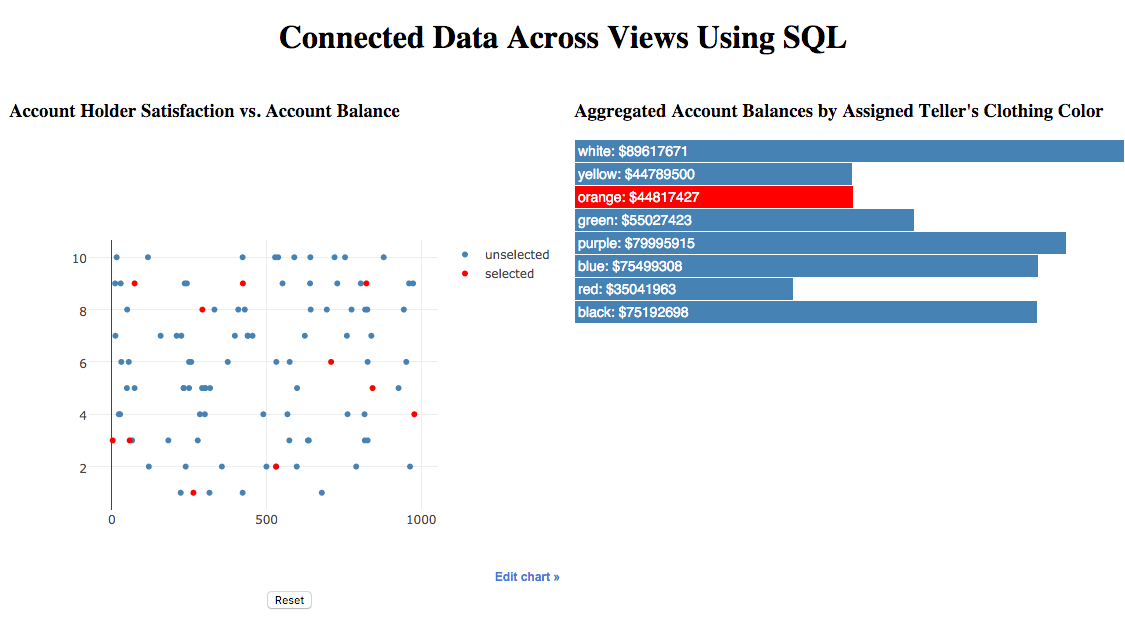
\includegraphics[width=\columnwidth]{figures/connect}
	\caption{A screenshot of the visualizations described in \autoref{connect}
	}
	\label{fig_connect}
\end{figure}
\subsubsection{Vega}
\subsubsection*{Scatter Plot ($V_1$, left view in Figure~\ref{fig_connect})}
\lstinputlisting[language=json, tabsize=2, emptylines=0]{../pgbench-connect/vega/scatterplot.json}
\subsubsection*{Bar Chart ($V_2$, right view in Figure~\ref{fig_connect})}
\lstinputlisting[language=json, tabsize=2, emptylines=0]{../pgbench-connect/vega/barchart.json}
\subsubsection{Alternative \#1 (whiteboarded on 11/12)}
Let $V_1$ be the scatter plot.
Let $V_2$ be the bar chart.
\begin{align*}
	V_1&= \mathlarger{\pi}_{circle}(\bf{accounts})\\
	S_1&= \mathlarger{\pi}_{circle}(\mathlarger{\sigma}_{P_1}(\bf{accounts}))\\
	V_2&= \mathlarger{\pi}_{rect}(\mathlarger{\gamma}_{ccolor, \text{SUM}(abalance)}(\bf{accounts}\bowtie{}\bf{tellers}))\\
	S_2&= \mathlarger{\pi}_{rect}(\mathlarger{\gamma}_{ccolor, \text{SUM}(abalance)}(\mathlarger{\sigma}_{P_2}(\bf{accounts}\bowtie{}\bf{tellers})))\\
	init()/reset()&:\\
	&: P_1 = P_2 = *\\
	&: S_1.color = S_2.color = \texttt{steelblue}\\
	click(V_2)&:\\
	&: P_2 = ``\text{WHERE}~ccolor=click.ccolor"\\
	&: P_1 = ``\text{WHERE}~aid~\text{IN~lineage}(S_2, \bf{accounts})"\\
	&: S_1.color = S_2.color = \texttt{red}\\
\end{align*}
\subsubsection{Alternative \#2}
Let $V_1$ be the scatter plot.
Let $V_2$ be the bar chart.
\begin{align*}
	V_1&= \mathlarger{\pi}_{circle}(\bf{accounts})\\
	S_1&= \mathlarger{\pi}_{circle}(\mathlarger{\sigma}_{P_2}(\bf{accounts}\bowtie{}\bf{tellers})))\\
	V_2&= \mathlarger{\pi}_{rect}(\mathlarger{\gamma}_{ccolor, \text{SUM}(abalance)}(\bf{accounts}\bowtie{}\bf{tellers}))\\
	S_2&= \mathlarger{\pi}_{rect}(\mathlarger{\gamma}_{ccolor, \text{SUM}(abalance)}(\mathlarger{\sigma}_{P_2}(\bf{accounts}\bowtie{}\bf{tellers})))\\
	init()/reset()&:\\
	&: P_2 = *\\
	&: S_1.color = S_2.color = \texttt{steelblue}\\
	click(V_2)&:\\
	&: P_2 = ``\text{WHERE}~ccolor=click.ccolor"\\
	&: S_1.color = S_2.color = \texttt{red}\\
\end{align*}
\subsection{Aggregation Filtering Using SQL \href{http://randy.cs.columbia.edu/lineage/pgbench-filter/pgbench.html}{(\underline{link})}}\label{filter}
\begin{figure}[H]
	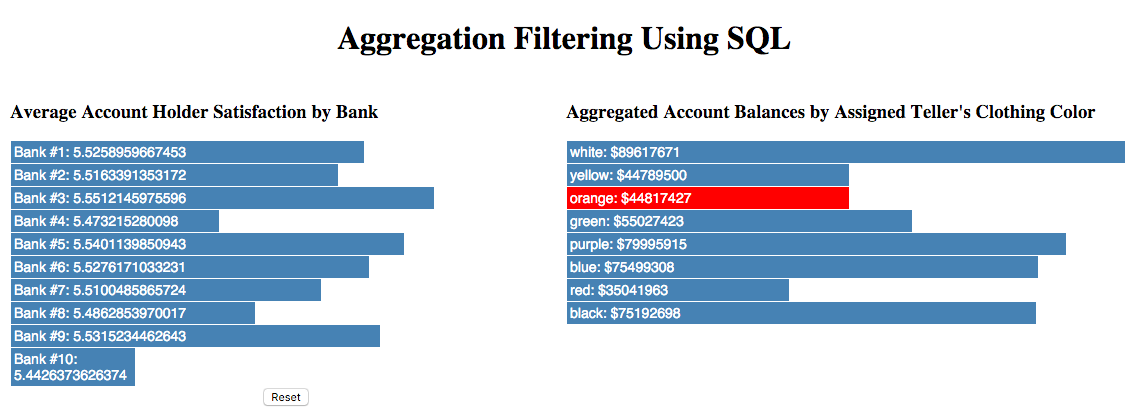
\includegraphics[width=\columnwidth]{figures/filter}
	\caption{A screenshot of the visualizations described in \autoref{filter}
	}
	\label{fig_filter}
\end{figure}
\subsubsection{Vega}
\subsubsection*{Satisfaction Bar Chart ($V_3$, left view in Figure~\ref{fig_filter})}
\lstinputlisting[language=json, tabsize=2, emptylines=0]{../pgbench-filter/vega/satisfactionbars.json}
\subsubsection*{Balance Bar Chart ($V_4$, right view in Figure~\ref{fig_filter})}
\lstinputlisting[language=json, tabsize=2, emptylines=0]{../pgbench-filter/vega/balancebars.json}
\subsubsection{Alternative}
Let $V_3$ be the satisfaction bar chart.
Let $V_4$ be the balance bar chart.
\begin{align*}
	V_3&= \mathlarger{\pi}_{rect}(\mathlarger{\gamma}_{bid, \text{AVG}(satisfaction)}(\bf{accounts}\bowtie{}\bf{tellers}))\\
	S_3&= \mathlarger{\pi}_{rect}(\mathlarger{\gamma}_{bid, \text{AVG}(satisfaction)}(\mathlarger{\sigma}_{P_3}(\bf{accounts}\bowtie{}\bf{tellers})))\\
	V_4&= \mathlarger{\pi}_{rect}(\mathlarger{\gamma}_{ccolor, \text{SUM}(abalance)}(\bf{accounts}\bowtie{}\bf{tellers}))\\
	S_4&= \mathlarger{\pi}_{rect}(\mathlarger{\gamma}_{ccolor, \text{SUM}(abalance)}(\mathlarger{\sigma}_{P_4}(\bf{accounts}\bowtie{}\bf{tellers})))\\
	init()/reset()&:\\
	&: P_3 = P_4 = *\\
	&: S_3.color = S_4.color = \texttt{steelblue}\\
	click(V_4)&:\\
	&: P_3 = P_4 = ``\text{WHERE}~ccolor=click.ccolor"\\
	&: S_3.color = S_4.color = \texttt{red}\\
\end{align*}
\pagebreak
\subsection{Vega vs. Alternatives}
\underline{Similarities}:
\begin{enumerate}
	\item Both descriptions are partially declarative and partially stateful.
	\item Both descriptions are event-driven, with state changes propagating up from interaction events to modify intermediate state, and eventually the rendered views (if necessary).
	\item The tables involved in rendering each view are immediately apparent from the description of the view/marks.
\end{enumerate}
\underline{Differences}:
\begin{enumerate}
	\item The alternate description is far more succinct than Vega.
	\item The alternate description leaves out many details.
		For example:
		\begin{itemize}
			\item scaling and position details contained in the projections $\mathlarger{\pi}_{circle}$ and $\mathlarger{\pi}_{rect}$,
			\item descriptive names for scales, predicates, and marks,
			\item scaling, position, and signal details corresponding to interaction events (this makes it difficult to specify predicates which depend on those events).
		\end{itemize}
\end{enumerate}
\subsection{Possible Indicators That Lineage Can Be Used for Optimization}
\begin{enumerate}
	\item The same tables are seen in the definitions for two different selection symbols.
	\item The predicate used to define one selection symbol contains another selection symbol.
	\item Two selection symbols use the same predicate.
\end{enumerate}
\subsection{Possible Indicators That Data Cubes Can Be Used for Optimization}
\begin{enumerate}
	\item The same exact mappings of the same tables are seen in the definitions for two different selection symbols.
\end{enumerate}

\bibliographystyle{refs}
\bibliography{refs}

\end{document}